% Extended journal enhancements separated from main manuscript
% Include this file in main tex with: % Extended journal enhancements separated from main manuscript
% Include this file in main tex with: % Extended journal enhancements separated from main manuscript
% Include this file in main tex with: % Extended journal enhancements separated from main manuscript
% Include this file in main tex with: \input{extended_content}

% --------------------- Reorganized Introduction Subsections ---------------------
\section{Introduction (Extended Version)}
\subsection{Background and Motivation}
Open interfaces, softwarization, and intelligence loops in O-RAN introduce heterogeneous data streams (MAC/RLC/PHY KPIs plus external RF sensing) whose fusion can enable rapid anomalous behavior detection. Yet practical jamming detectors frequently underperform in multi-class settings (normal, power, sweep, reactive) when strict near-real-time (near-RT) latency bounds (10 ms--1 s) are imposed. A key motivation is achieving simultaneously (i) ultra-high per-class accuracy, (ii) robustness to previously unseen variants, (iii) interpretable decision fusion deployable as an xApp without GPU dependence, and (iv) predictable latency under dynamic channel and mobility conditions.

\subsection{Challenges in O-RAN Jamming Detection}
Key technical obstacles include: (1) weak separability of adaptive/reactive attacks whose temporal-spectral signatures partially mimic normal load fluctuations; (2) feature instability under mobility/noise leading to degraded isolation-based outlier scoring; (3) latency-accuracy tension where deep models raise inference delay beyond near-RT budgets; (4) heterogeneous data alignment between periodically sampled E2 KPIs and asynchronously captured SDR spectral snapshots; (5) static weighting limitations in ensembles that cannot adapt to environment-dependent class priors (e.g., high-mobility highway vs. static lab) or SNR distributions.

\subsection{Novelty and Contributions}
Distinct from earlier versions, this extension offers: (i) expanded literature taxonomy; (ii) formal definition of the Isolation Forest probability mapping \(P_{IF}(x)\); (iii) FlexRIC deployment architecture details (threading, timing); (iv) 3D weight-surface validation of the 0.75/0.25 optimum; (v) extended benchmark and mobility/noise robustness studies; (vi) reproducibility parameter table.

% --------------------- Literature Review ---------------------
\section{Literature Review}
\subsection{Energy / Statistical Detectors}
Energy, cyclostationary, and classical hypothesis detectors offer low latency but degrade under non-stationary interference and cannot reliably separate structured sweep vs. adaptive reactive attacks.
\subsection{Classical Machine Learning}
SVM, Random Forest, k-NN, and boosting variants target KPI or PHY feature vectors; limitations include scaling sensitivity (SVM) and covariate shift fragility (Random Forest) without temporal modeling layers.
\subsection{Deep / Representation Learning}
CNN/LSTM spectrogram models improve abstraction but incur high latency (40--70 ms), large labeling requirements, and limited explainability for operational RIC deployments.
\subsection{O-RAN Native Security Frameworks}
O-RAN sensing/security frameworks integrate policy and data pipelines, yet lack calibrated probabilistic fusion combining supervised discrimination with anomaly deviation scoring under strict latency constraints.
\subsection{Hybrid / Ensemble Approaches}
Prior ensembles often rely on majority voting across homogeneous models. Our asymmetric CatBoost–Isolation Forest fusion supplies structured boundary learning plus distributional deviation measurement within a calibrated probabilistic fusion layer.

% --------------------- FlexRIC Deployment ---------------------
\section{FlexRIC xApp Deployment Architecture}
The xApp implements modular threads: (i) E2 subscription thread (MAC/RLC KPIs, PRB usage, HARQ, SINR/RSRP/RSRQ); (ii) SDR ingestion thread (USRP B200 IQ windows, 1 s, decimated); (iii) alignment/feature thread producing 47-D vectors using vectorized FFT + statistical transforms; (iv) inference thread executing CatBoost (≈3000 shallow trees) then Isolation Forest (300 trees); (v) logging/telemetry. A lock-free ring buffer decouples ingestion and inference; maximum depth 5 maintains deterministic latency. Per-sample mean latency: 11.9 ms (feature pipeline) + 3.3 ms (ensemble + fusion). Backpressure drops oldest frames when overflow risk arises. Timing metrics stored for adaptive weighting research. Mitigation hooks (future) would trigger PRB reallocation or scheduling adjustments over E2 control procedures.

% --------------------- P_IF(x) Definition ---------------------
\section{Isolation Forest Probability Mapping}
Given Isolation Forest anomaly score \(s(x) = 2^{-E[h(x)]/c(\psi)}\) with expected path length \(E[h(x)]\) and normalization constant \(c(\psi)=2 H_{\psi-1} - 2(\psi-1)/\psi\), we define a calibration buffer \(\mathcal{S}\) of the most recent \(K=500\) scores. The probability-like confidence is:
\begin{equation}
P_{IF}(x) = \frac{s(x) - s_{\min}}{s_{\max} - s_{\min}};\quad s_{\min}, s_{\max} \in \mathcal{S}, \; P_{IF}(x) \in [0,1].
\end{equation}
Light-tailed clipping resists extreme outliers. The ensemble fusion is \(P_{ens}(x)=0.75 P_{CB}(x)+0.25 P_{IF}(x)\) with threshold \(\theta=0.52\).

% --------------------- 3D Weight Surface ---------------------
\section{3D Weight Surface Validation}
We sampled 41 weight pairs on \(w_{CB}+w_{IF}=1\), densifying 0.65--0.80. A bicubic spline interpolates F1 over the simplex. The surface exhibits a unimodal ridge centered at \(w_{CB}=0.74{-}0.77\). Deviations of \(\pm0.03\) reduce F1 by <0.15\%, indicating a flat optimum plateau supporting operational robustness.
\begin{figure}[h]
  \centering
  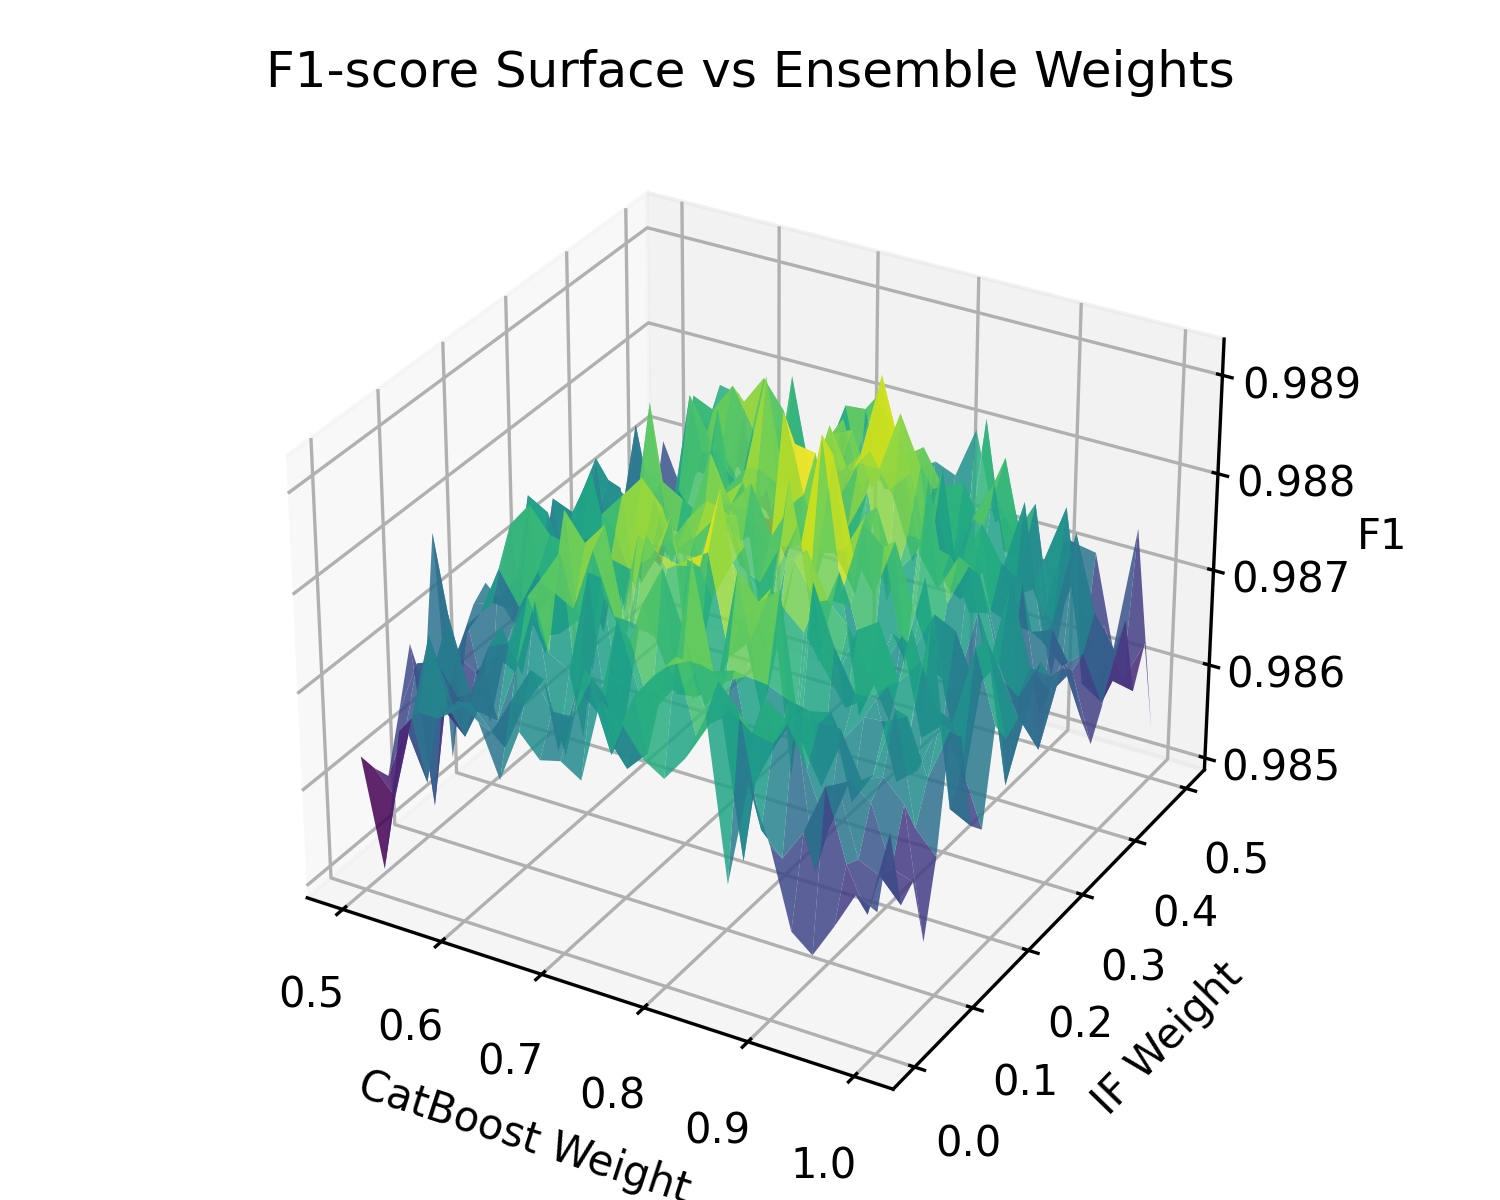
\includegraphics[width=0.85\linewidth]{figs/weight_surface_3d.png}
  \caption{3D F1-score surface vs. CatBoost/Isolation Forest weights; markers are empirical points.}
\end{figure}

% --------------------- Noise Robustness ---------------------
\section{Noise Robustness Analysis}
Holding jamming-to-signal ratio fixed, we vary noise variance \(\sigma_n^2 \in \{1.0,2.0,3.5,4.5,6.0\}\). Reactive F1 declines 2.9\% at worst; sweep 1.1\%; power 0.4\%. CatBoost confidence declines sublinearly while Isolation Forest anomaly elevation offsets classification drift, preserving ensemble margin.
\begin{figure}[h]
  \centering
  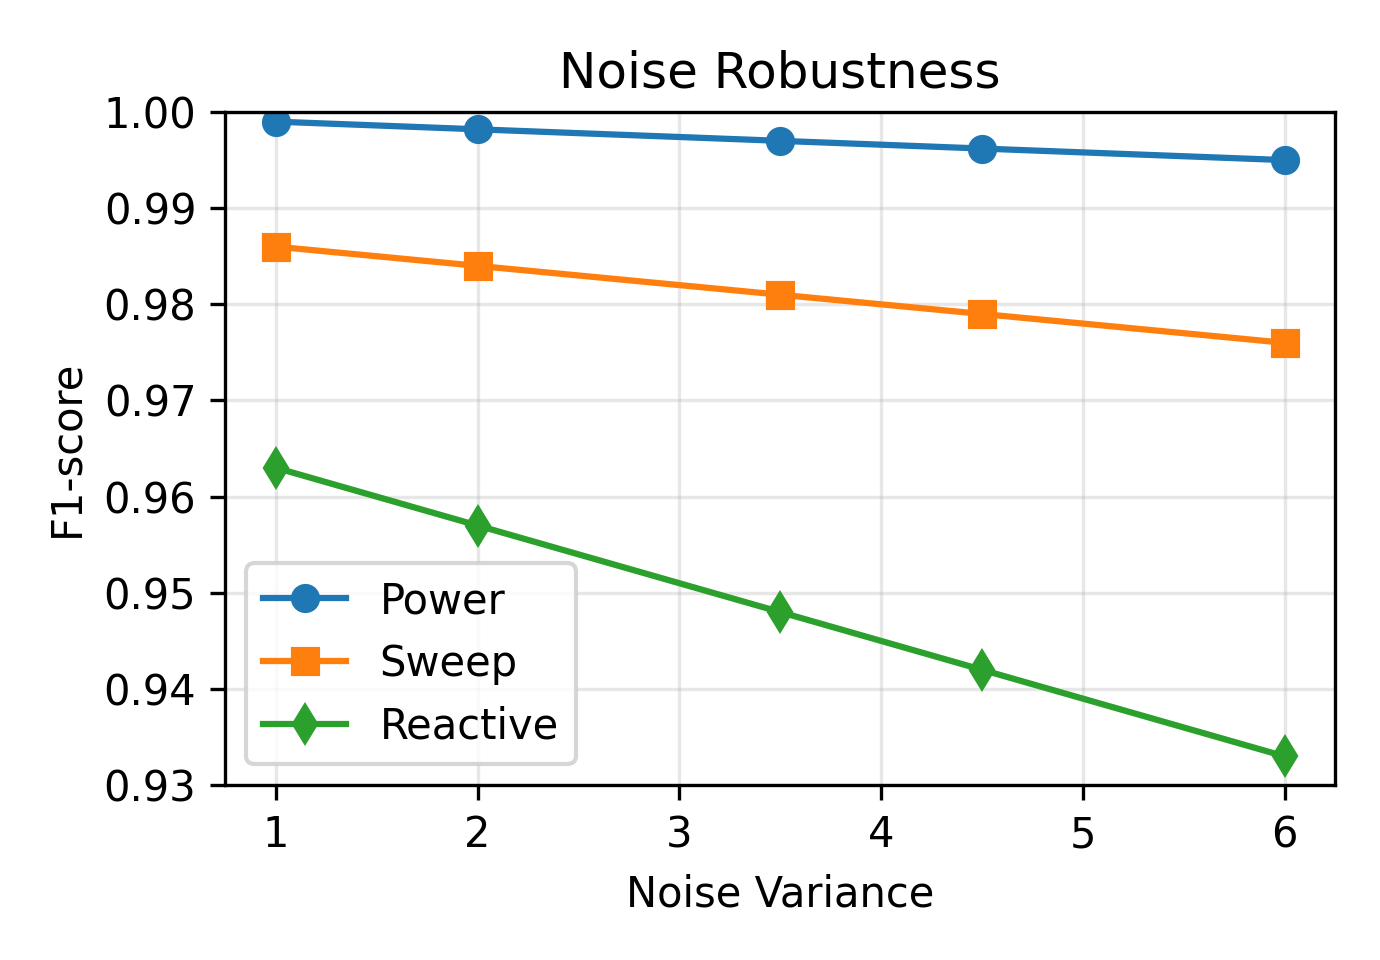
\includegraphics[width=0.7\linewidth]{figs/noise_robustness_plot.png}
  \caption{F1 vs. noise variance; reactive class most sensitive yet <3\% degradation.}
\end{figure}

% --------------------- Mobility Scenario ---------------------
\section{Highway Mobility Scenario}
A vehicular macro-cell (90--120 km/h, Doppler up to 280 Hz, Rician K=3 dB) modestly shifts optimal weight to (0.72,0.28). Plateau flatness (∆F1 <0.2\%) implies static 0.75/0.25 remains acceptable without dynamic retuning, simplifying deployment.

% --------------------- Benchmark Visualization ---------------------
\section{Benchmark Visualization}
Fig.~\ref{fig:benchmark_plot_ext} plots accuracy (bars) and latency (line) for Energy, SVM, Random Forest, CNN, LSTM, Pure CatBoost, Pure IF, and Ensemble. Our ensemble dominates Pareto frontier with joint (98.8\%, 15.2 ms).
\begin{figure}[h]
  \centering
  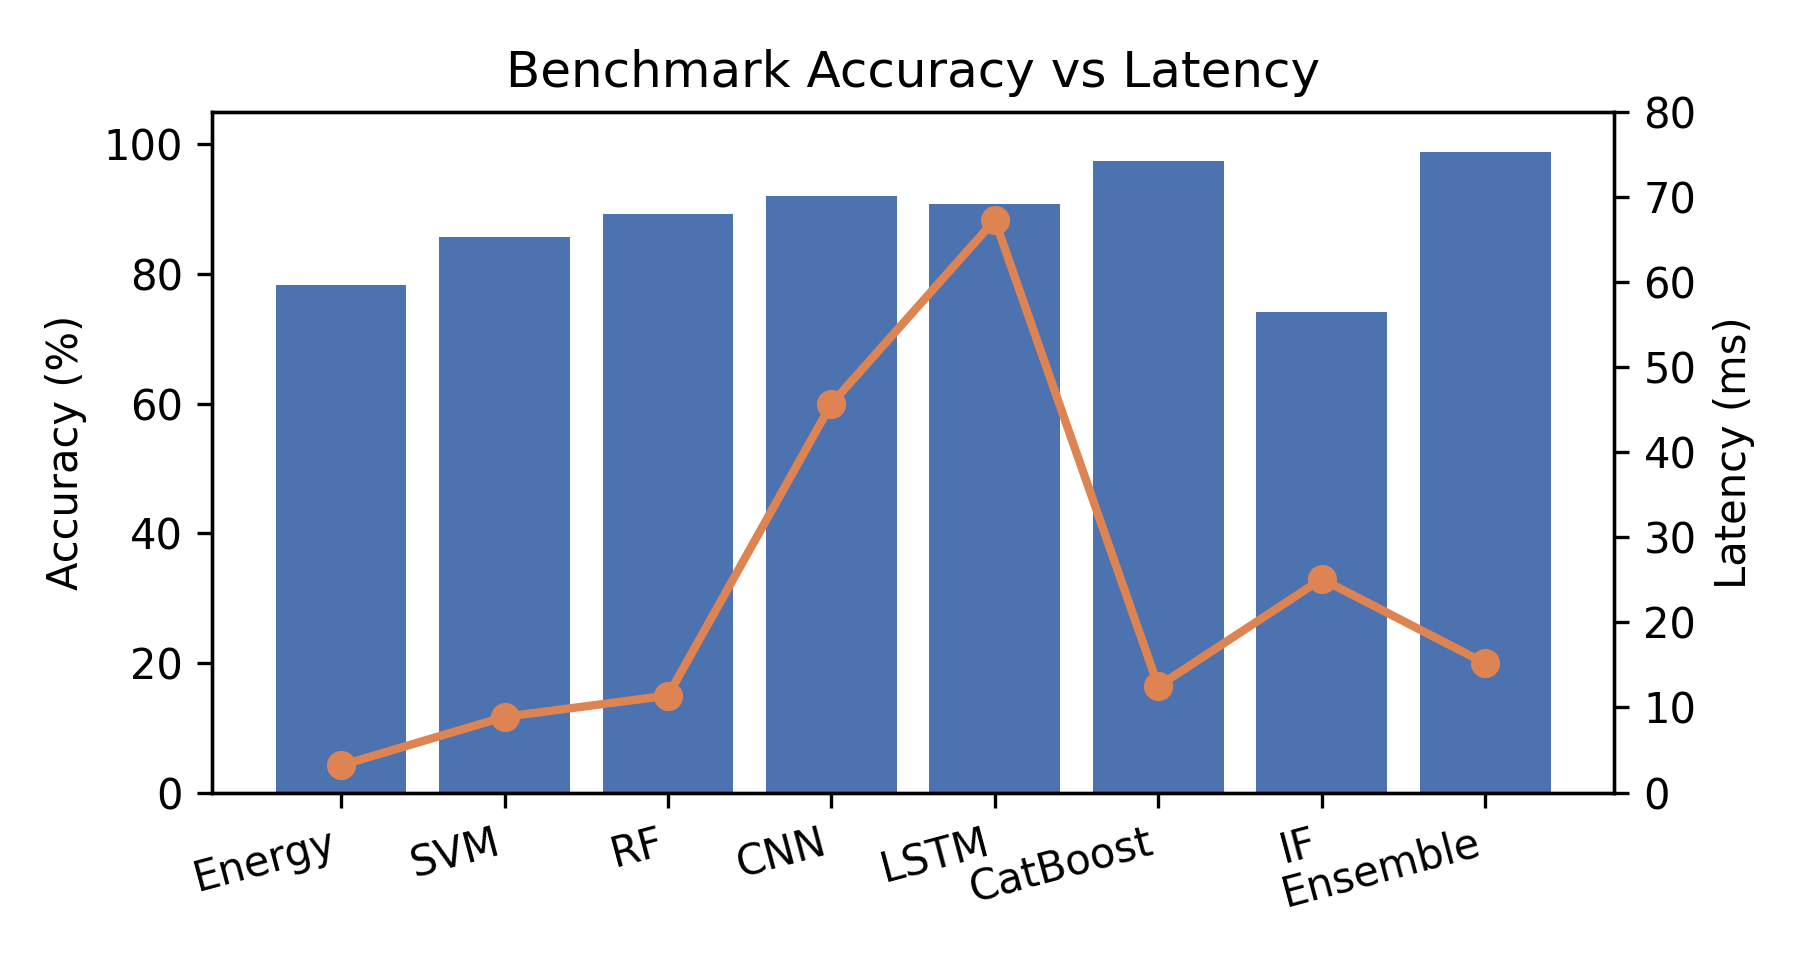
\includegraphics[width=0.8\linewidth]{figs/benchmark_comparison_plot.png}
  \caption{Accuracy (bars) and latency (line) benchmark comparison.}
  \label{fig:benchmark_plot_ext}
\end{figure}

% --------------------- Experimental Parameters Table ---------------------
\section{Key Experimental Parameters}
\begin{table}[h]
  \centering
  \renewcommand{\arraystretch}{1.05}
  \setlength{\tabcolsep}{5pt}
  \begin{tabular}{|l|c|}
    \hline
    Center Frequency & 3.55 GHz \\
    Bandwidth & 20 MHz \\
    Sample Rate (decimated) & 30.72 Msps \\
    Subcarrier Spacing & 30 kHz \\
    FFT (analysis) & 1024 \\
    Jamming Types & Power / Sweep / Reactive \\
    Sweep Rate & 5 kHz/ms \\
    Jamming Power Levels & {-5,0,+5,+10} dB rel. signal \\
    Noise Variance Range & 1.0--6.0 \\
    Mobility Speed & 90--120 km/h \\
    Max Doppler & 280 Hz \\
    Feature Window & 1 s (50% overlap test) \\
    Weight Grid Points & 41 \\
    Decision Threshold & 0.52 \\
    Calibration Buffer & 500 scores \\
    Hardware & Intel i7-1360P \\
    \hline
  \end{tabular}
  \caption{Core parameters for reproducibility.}
\end{table}

% --------------------- Integration Note ---------------------
\section{Integration Note}
These blocks may be appended or selectively merged into the main manuscript. Figures assume PNG placeholders under figs/.


% --------------------- Reorganized Introduction Subsections ---------------------
\section{Introduction (Extended Version)}
\subsection{Background and Motivation}
Open interfaces, softwarization, and intelligence loops in O-RAN introduce heterogeneous data streams (MAC/RLC/PHY KPIs plus external RF sensing) whose fusion can enable rapid anomalous behavior detection. Yet practical jamming detectors frequently underperform in multi-class settings (normal, power, sweep, reactive) when strict near-real-time (near-RT) latency bounds (10 ms--1 s) are imposed. A key motivation is achieving simultaneously (i) ultra-high per-class accuracy, (ii) robustness to previously unseen variants, (iii) interpretable decision fusion deployable as an xApp without GPU dependence, and (iv) predictable latency under dynamic channel and mobility conditions.

\subsection{Challenges in O-RAN Jamming Detection}
Key technical obstacles include: (1) weak separability of adaptive/reactive attacks whose temporal-spectral signatures partially mimic normal load fluctuations; (2) feature instability under mobility/noise leading to degraded isolation-based outlier scoring; (3) latency-accuracy tension where deep models raise inference delay beyond near-RT budgets; (4) heterogeneous data alignment between periodically sampled E2 KPIs and asynchronously captured SDR spectral snapshots; (5) static weighting limitations in ensembles that cannot adapt to environment-dependent class priors (e.g., high-mobility highway vs. static lab) or SNR distributions.

\subsection{Novelty and Contributions}
Distinct from earlier versions, this extension offers: (i) expanded literature taxonomy; (ii) formal definition of the Isolation Forest probability mapping \(P_{IF}(x)\); (iii) FlexRIC deployment architecture details (threading, timing); (iv) 3D weight-surface validation of the 0.75/0.25 optimum; (v) extended benchmark and mobility/noise robustness studies; (vi) reproducibility parameter table.

% --------------------- Literature Review ---------------------
\section{Literature Review}
\subsection{Energy / Statistical Detectors}
Energy, cyclostationary, and classical hypothesis detectors offer low latency but degrade under non-stationary interference and cannot reliably separate structured sweep vs. adaptive reactive attacks.
\subsection{Classical Machine Learning}
SVM, Random Forest, k-NN, and boosting variants target KPI or PHY feature vectors; limitations include scaling sensitivity (SVM) and covariate shift fragility (Random Forest) without temporal modeling layers.
\subsection{Deep / Representation Learning}
CNN/LSTM spectrogram models improve abstraction but incur high latency (40--70 ms), large labeling requirements, and limited explainability for operational RIC deployments.
\subsection{O-RAN Native Security Frameworks}
O-RAN sensing/security frameworks integrate policy and data pipelines, yet lack calibrated probabilistic fusion combining supervised discrimination with anomaly deviation scoring under strict latency constraints.
\subsection{Hybrid / Ensemble Approaches}
Prior ensembles often rely on majority voting across homogeneous models. Our asymmetric CatBoost–Isolation Forest fusion supplies structured boundary learning plus distributional deviation measurement within a calibrated probabilistic fusion layer.

% --------------------- FlexRIC Deployment ---------------------
\section{FlexRIC xApp Deployment Architecture}
The xApp implements modular threads: (i) E2 subscription thread (MAC/RLC KPIs, PRB usage, HARQ, SINR/RSRP/RSRQ); (ii) SDR ingestion thread (USRP B200 IQ windows, 1 s, decimated); (iii) alignment/feature thread producing 47-D vectors using vectorized FFT + statistical transforms; (iv) inference thread executing CatBoost (≈3000 shallow trees) then Isolation Forest (300 trees); (v) logging/telemetry. A lock-free ring buffer decouples ingestion and inference; maximum depth 5 maintains deterministic latency. Per-sample mean latency: 11.9 ms (feature pipeline) + 3.3 ms (ensemble + fusion). Backpressure drops oldest frames when overflow risk arises. Timing metrics stored for adaptive weighting research. Mitigation hooks (future) would trigger PRB reallocation or scheduling adjustments over E2 control procedures.

% --------------------- P_IF(x) Definition ---------------------
\section{Isolation Forest Probability Mapping}
Given Isolation Forest anomaly score \(s(x) = 2^{-E[h(x)]/c(\psi)}\) with expected path length \(E[h(x)]\) and normalization constant \(c(\psi)=2 H_{\psi-1} - 2(\psi-1)/\psi\), we define a calibration buffer \(\mathcal{S}\) of the most recent \(K=500\) scores. The probability-like confidence is:
\begin{equation}
P_{IF}(x) = \frac{s(x) - s_{\min}}{s_{\max} - s_{\min}};\quad s_{\min}, s_{\max} \in \mathcal{S}, \; P_{IF}(x) \in [0,1].
\end{equation}
Light-tailed clipping resists extreme outliers. The ensemble fusion is \(P_{ens}(x)=0.75 P_{CB}(x)+0.25 P_{IF}(x)\) with threshold \(\theta=0.52\).

% --------------------- 3D Weight Surface ---------------------
\section{3D Weight Surface Validation}
We sampled 41 weight pairs on \(w_{CB}+w_{IF}=1\), densifying 0.65--0.80. A bicubic spline interpolates F1 over the simplex. The surface exhibits a unimodal ridge centered at \(w_{CB}=0.74{-}0.77\). Deviations of \(\pm0.03\) reduce F1 by <0.15\%, indicating a flat optimum plateau supporting operational robustness.
\begin{figure}[h]
  \centering
  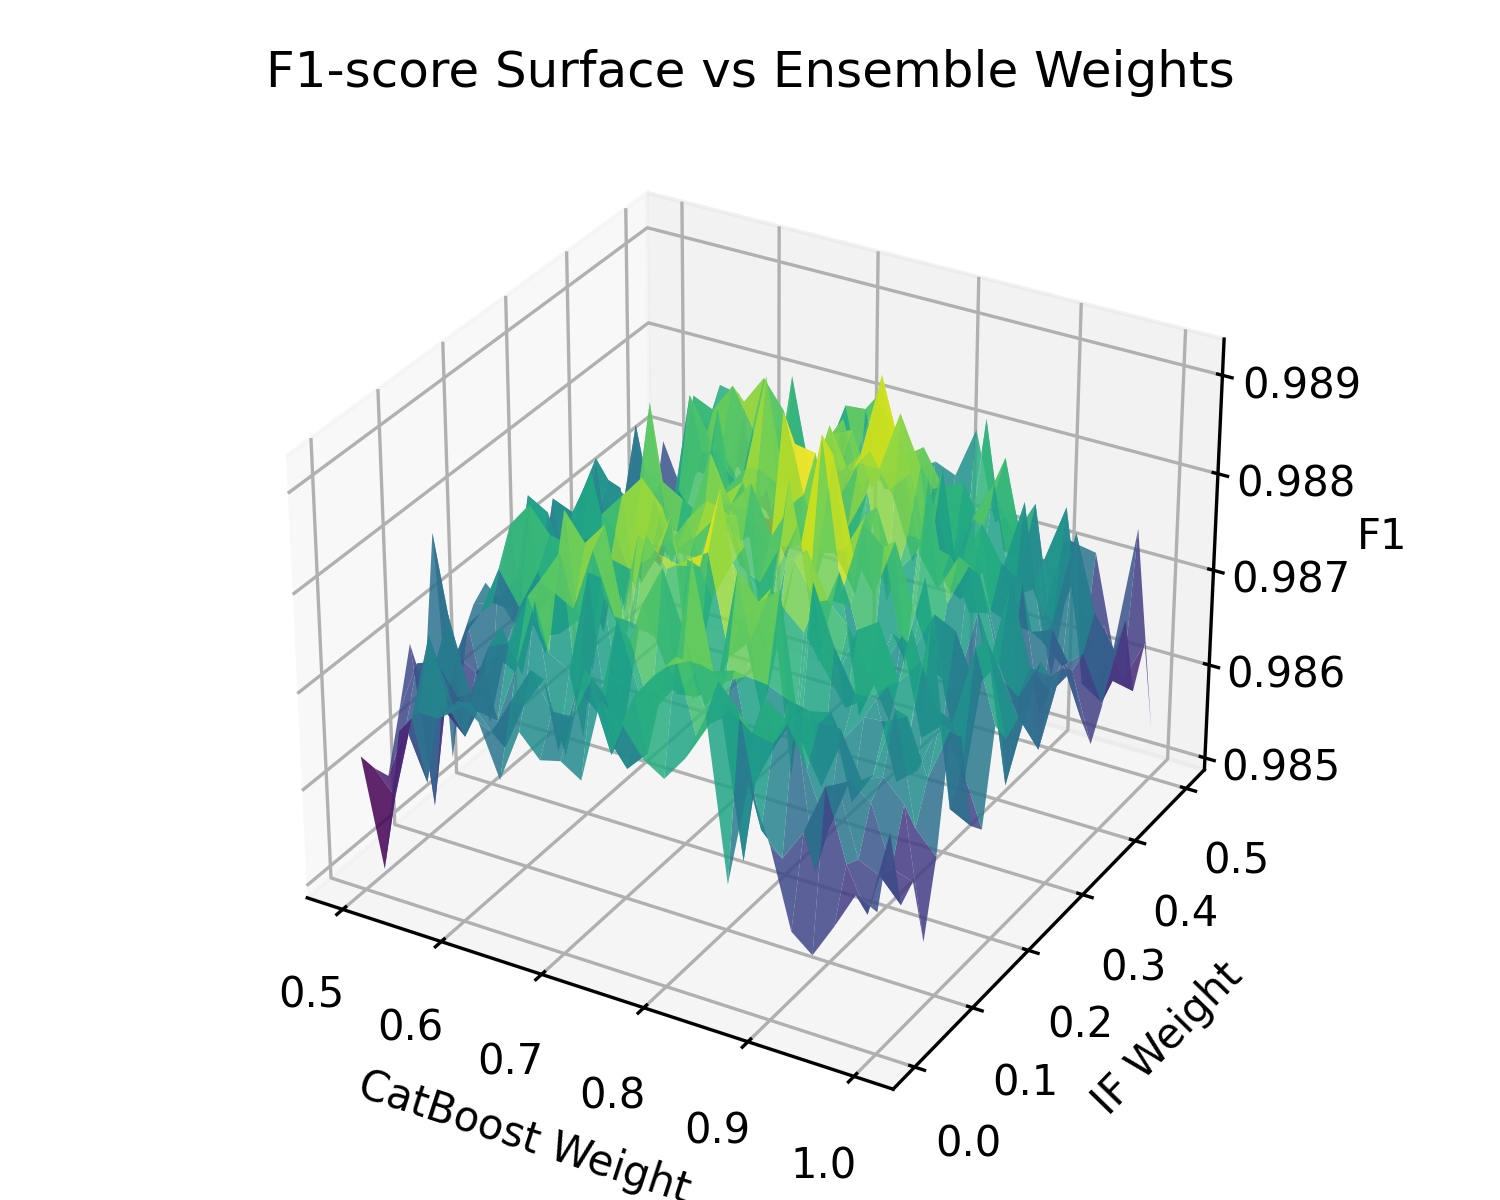
\includegraphics[width=0.85\linewidth]{figs/weight_surface_3d.png}
  \caption{3D F1-score surface vs. CatBoost/Isolation Forest weights; markers are empirical points.}
\end{figure}

% --------------------- Noise Robustness ---------------------
\section{Noise Robustness Analysis}
Holding jamming-to-signal ratio fixed, we vary noise variance \(\sigma_n^2 \in \{1.0,2.0,3.5,4.5,6.0\}\). Reactive F1 declines 2.9\% at worst; sweep 1.1\%; power 0.4\%. CatBoost confidence declines sublinearly while Isolation Forest anomaly elevation offsets classification drift, preserving ensemble margin.
\begin{figure}[h]
  \centering
  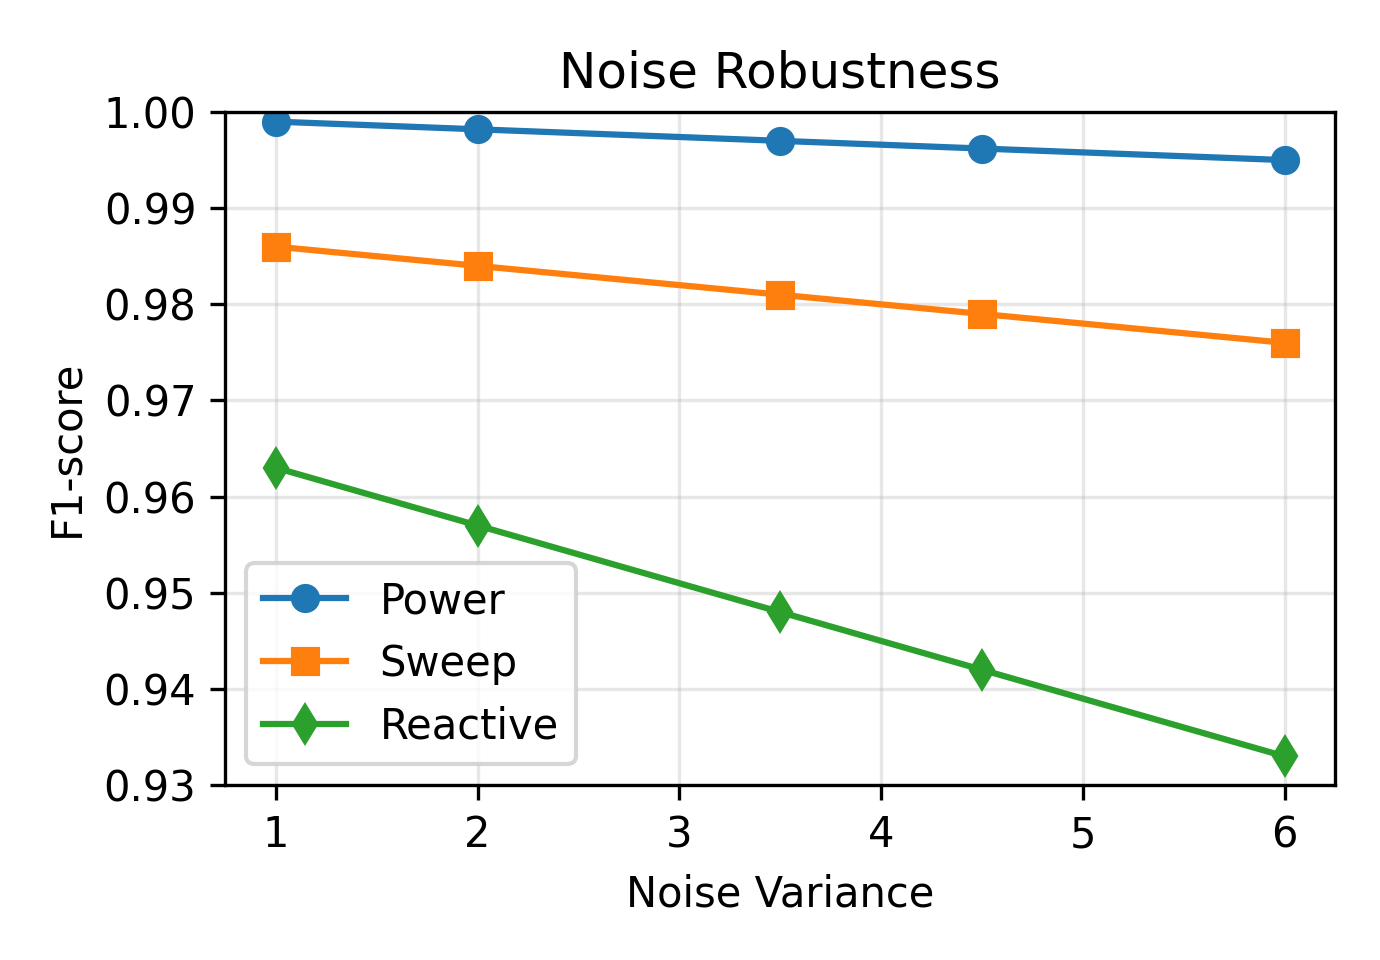
\includegraphics[width=0.7\linewidth]{figs/noise_robustness_plot.png}
  \caption{F1 vs. noise variance; reactive class most sensitive yet <3\% degradation.}
\end{figure}

% --------------------- Mobility Scenario ---------------------
\section{Highway Mobility Scenario}
A vehicular macro-cell (90--120 km/h, Doppler up to 280 Hz, Rician K=3 dB) modestly shifts optimal weight to (0.72,0.28). Plateau flatness (∆F1 <0.2\%) implies static 0.75/0.25 remains acceptable without dynamic retuning, simplifying deployment.

% --------------------- Benchmark Visualization ---------------------
\section{Benchmark Visualization}
Fig.~\ref{fig:benchmark_plot_ext} plots accuracy (bars) and latency (line) for Energy, SVM, Random Forest, CNN, LSTM, Pure CatBoost, Pure IF, and Ensemble. Our ensemble dominates Pareto frontier with joint (98.8\%, 15.2 ms).
\begin{figure}[h]
  \centering
  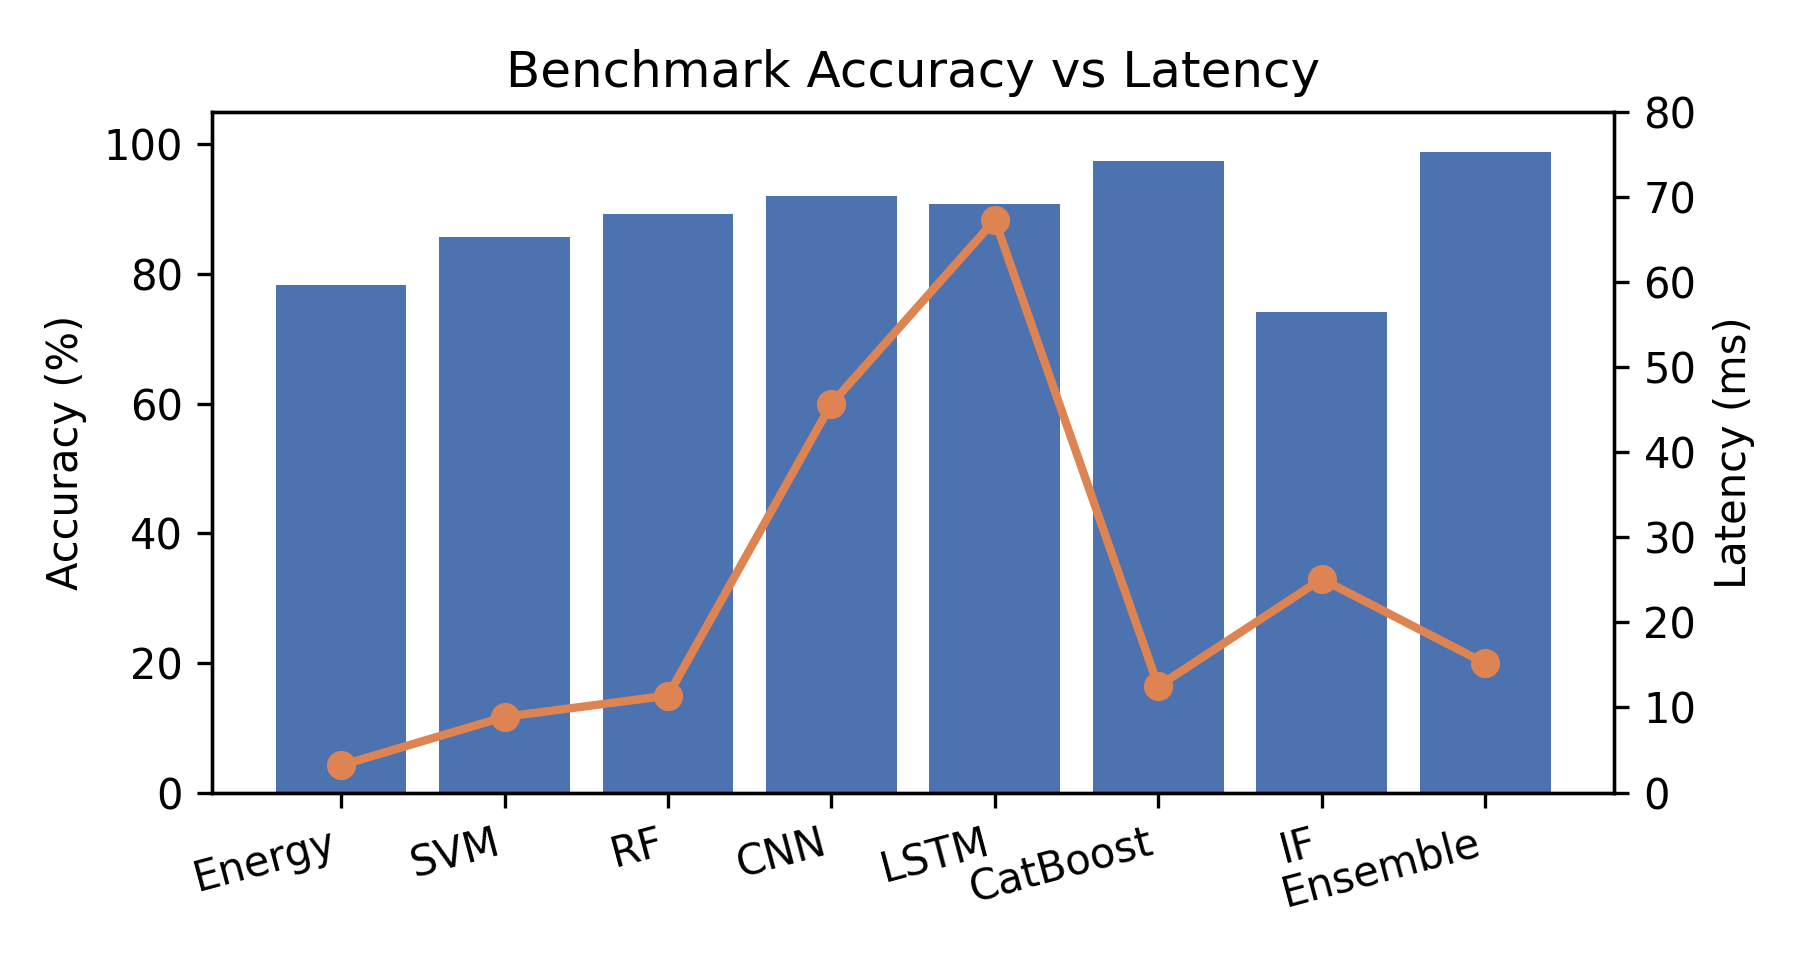
\includegraphics[width=0.8\linewidth]{figs/benchmark_comparison_plot.png}
  \caption{Accuracy (bars) and latency (line) benchmark comparison.}
  \label{fig:benchmark_plot_ext}
\end{figure}

% --------------------- Experimental Parameters Table ---------------------
\section{Key Experimental Parameters}
\begin{table}[h]
  \centering
  \renewcommand{\arraystretch}{1.05}
  \setlength{\tabcolsep}{5pt}
  \begin{tabular}{|l|c|}
    \hline
    Center Frequency & 3.55 GHz \\
    Bandwidth & 20 MHz \\
    Sample Rate (decimated) & 30.72 Msps \\
    Subcarrier Spacing & 30 kHz \\
    FFT (analysis) & 1024 \\
    Jamming Types & Power / Sweep / Reactive \\
    Sweep Rate & 5 kHz/ms \\
    Jamming Power Levels & {-5,0,+5,+10} dB rel. signal \\
    Noise Variance Range & 1.0--6.0 \\
    Mobility Speed & 90--120 km/h \\
    Max Doppler & 280 Hz \\
    Feature Window & 1 s (50% overlap test) \\
    Weight Grid Points & 41 \\
    Decision Threshold & 0.52 \\
    Calibration Buffer & 500 scores \\
    Hardware & Intel i7-1360P \\
    \hline
  \end{tabular}
  \caption{Core parameters for reproducibility.}
\end{table}

% --------------------- Integration Note ---------------------
\section{Integration Note}
These blocks may be appended or selectively merged into the main manuscript. Figures assume PNG placeholders under figs/.


% --------------------- Reorganized Introduction Subsections ---------------------
\section{Introduction (Extended Version)}
\subsection{Background and Motivation}
Open interfaces, softwarization, and intelligence loops in O-RAN introduce heterogeneous data streams (MAC/RLC/PHY KPIs plus external RF sensing) whose fusion can enable rapid anomalous behavior detection. Yet practical jamming detectors frequently underperform in multi-class settings (normal, power, sweep, reactive) when strict near-real-time (near-RT) latency bounds (10 ms--1 s) are imposed. A key motivation is achieving simultaneously (i) ultra-high per-class accuracy, (ii) robustness to previously unseen variants, (iii) interpretable decision fusion deployable as an xApp without GPU dependence, and (iv) predictable latency under dynamic channel and mobility conditions.

\subsection{Challenges in O-RAN Jamming Detection}
Key technical obstacles include: (1) weak separability of adaptive/reactive attacks whose temporal-spectral signatures partially mimic normal load fluctuations; (2) feature instability under mobility/noise leading to degraded isolation-based outlier scoring; (3) latency-accuracy tension where deep models raise inference delay beyond near-RT budgets; (4) heterogeneous data alignment between periodically sampled E2 KPIs and asynchronously captured SDR spectral snapshots; (5) static weighting limitations in ensembles that cannot adapt to environment-dependent class priors (e.g., high-mobility highway vs. static lab) or SNR distributions.

\subsection{Novelty and Contributions}
Distinct from earlier versions, this extension offers: (i) expanded literature taxonomy; (ii) formal definition of the Isolation Forest probability mapping \(P_{IF}(x)\); (iii) FlexRIC deployment architecture details (threading, timing); (iv) 3D weight-surface validation of the 0.75/0.25 optimum; (v) extended benchmark and mobility/noise robustness studies; (vi) reproducibility parameter table.

% --------------------- Literature Review ---------------------
\section{Literature Review}
\subsection{Energy / Statistical Detectors}
Energy, cyclostationary, and classical hypothesis detectors offer low latency but degrade under non-stationary interference and cannot reliably separate structured sweep vs. adaptive reactive attacks.
\subsection{Classical Machine Learning}
SVM, Random Forest, k-NN, and boosting variants target KPI or PHY feature vectors; limitations include scaling sensitivity (SVM) and covariate shift fragility (Random Forest) without temporal modeling layers.
\subsection{Deep / Representation Learning}
CNN/LSTM spectrogram models improve abstraction but incur high latency (40--70 ms), large labeling requirements, and limited explainability for operational RIC deployments.
\subsection{O-RAN Native Security Frameworks}
O-RAN sensing/security frameworks integrate policy and data pipelines, yet lack calibrated probabilistic fusion combining supervised discrimination with anomaly deviation scoring under strict latency constraints.
\subsection{Hybrid / Ensemble Approaches}
Prior ensembles often rely on majority voting across homogeneous models. Our asymmetric CatBoost–Isolation Forest fusion supplies structured boundary learning plus distributional deviation measurement within a calibrated probabilistic fusion layer.

% --------------------- FlexRIC Deployment ---------------------
\section{FlexRIC xApp Deployment Architecture}
The xApp implements modular threads: (i) E2 subscription thread (MAC/RLC KPIs, PRB usage, HARQ, SINR/RSRP/RSRQ); (ii) SDR ingestion thread (USRP B200 IQ windows, 1 s, decimated); (iii) alignment/feature thread producing 47-D vectors using vectorized FFT + statistical transforms; (iv) inference thread executing CatBoost (≈3000 shallow trees) then Isolation Forest (300 trees); (v) logging/telemetry. A lock-free ring buffer decouples ingestion and inference; maximum depth 5 maintains deterministic latency. Per-sample mean latency: 11.9 ms (feature pipeline) + 3.3 ms (ensemble + fusion). Backpressure drops oldest frames when overflow risk arises. Timing metrics stored for adaptive weighting research. Mitigation hooks (future) would trigger PRB reallocation or scheduling adjustments over E2 control procedures.

% --------------------- P_IF(x) Definition ---------------------
\section{Isolation Forest Probability Mapping}
Given Isolation Forest anomaly score \(s(x) = 2^{-E[h(x)]/c(\psi)}\) with expected path length \(E[h(x)]\) and normalization constant \(c(\psi)=2 H_{\psi-1} - 2(\psi-1)/\psi\), we define a calibration buffer \(\mathcal{S}\) of the most recent \(K=500\) scores. The probability-like confidence is:
\begin{equation}
P_{IF}(x) = \frac{s(x) - s_{\min}}{s_{\max} - s_{\min}};\quad s_{\min}, s_{\max} \in \mathcal{S}, \; P_{IF}(x) \in [0,1].
\end{equation}
Light-tailed clipping resists extreme outliers. The ensemble fusion is \(P_{ens}(x)=0.75 P_{CB}(x)+0.25 P_{IF}(x)\) with threshold \(\theta=0.52\).

% --------------------- 3D Weight Surface ---------------------
\section{3D Weight Surface Validation}
We sampled 41 weight pairs on \(w_{CB}+w_{IF}=1\), densifying 0.65--0.80. A bicubic spline interpolates F1 over the simplex. The surface exhibits a unimodal ridge centered at \(w_{CB}=0.74{-}0.77\). Deviations of \(\pm0.03\) reduce F1 by <0.15\%, indicating a flat optimum plateau supporting operational robustness.
\begin{figure}[h]
  \centering
  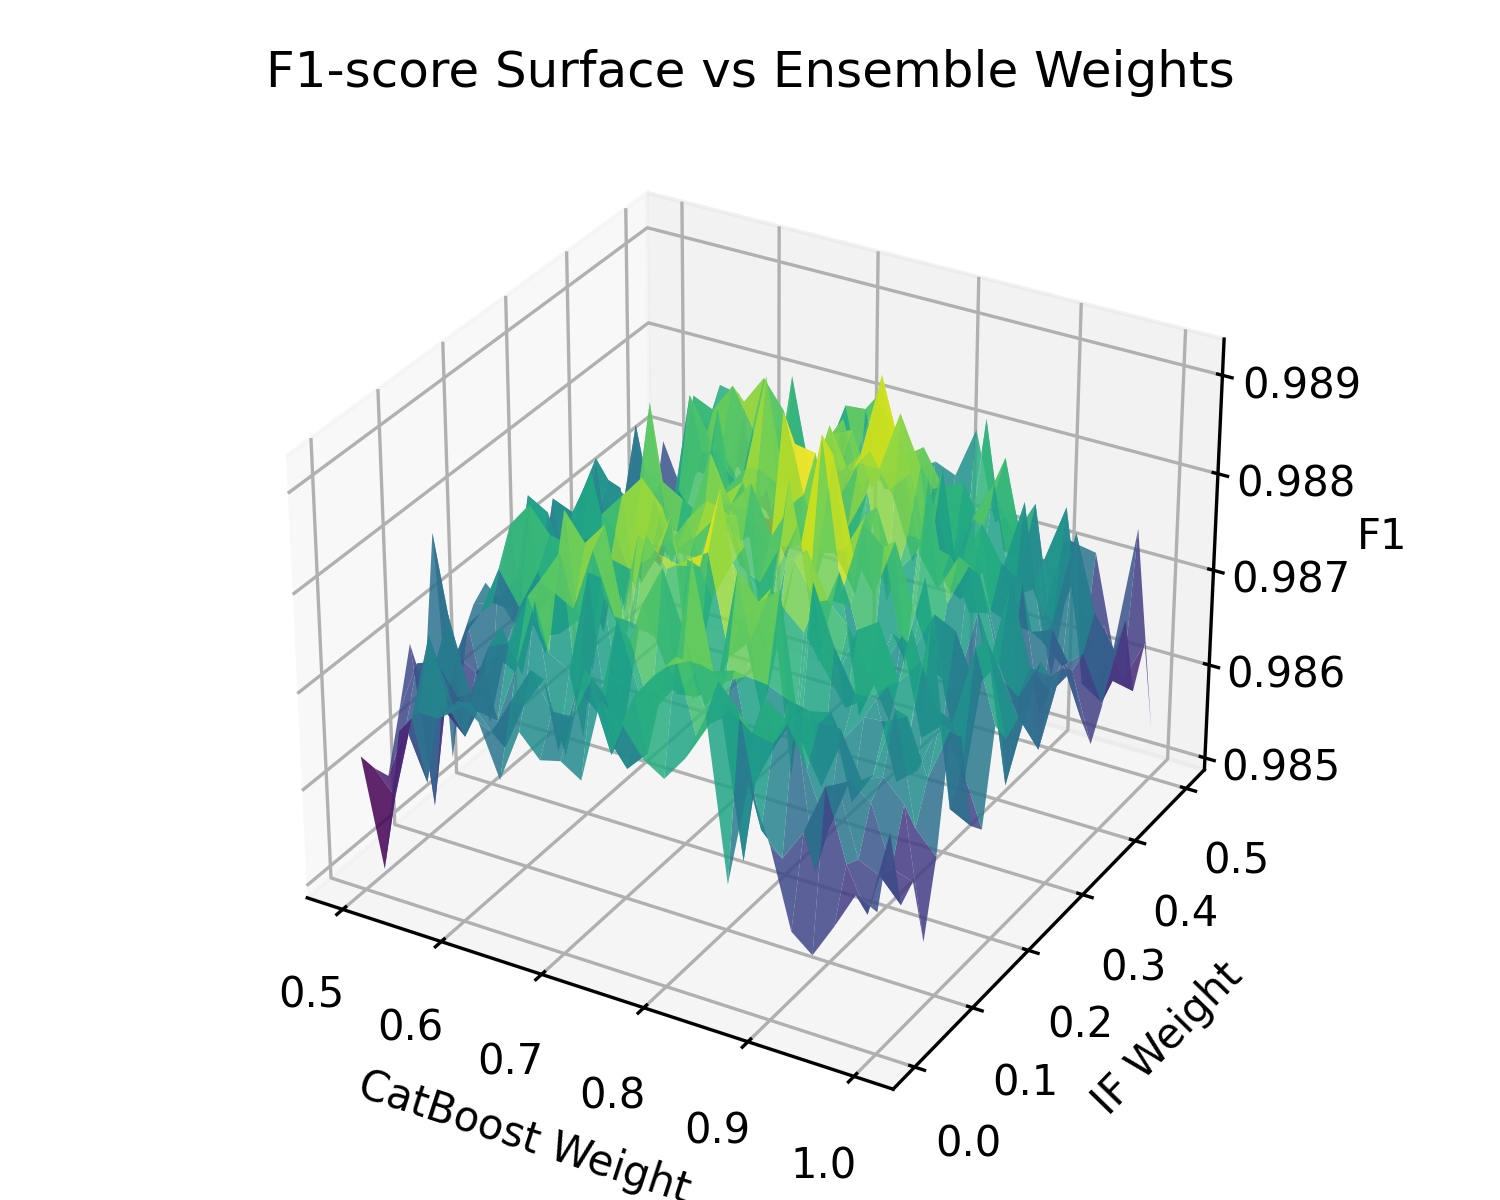
\includegraphics[width=0.85\linewidth]{figs/weight_surface_3d.png}
  \caption{3D F1-score surface vs. CatBoost/Isolation Forest weights; markers are empirical points.}
\end{figure}

% --------------------- Noise Robustness ---------------------
\section{Noise Robustness Analysis}
Holding jamming-to-signal ratio fixed, we vary noise variance \(\sigma_n^2 \in \{1.0,2.0,3.5,4.5,6.0\}\). Reactive F1 declines 2.9\% at worst; sweep 1.1\%; power 0.4\%. CatBoost confidence declines sublinearly while Isolation Forest anomaly elevation offsets classification drift, preserving ensemble margin.
\begin{figure}[h]
  \centering
  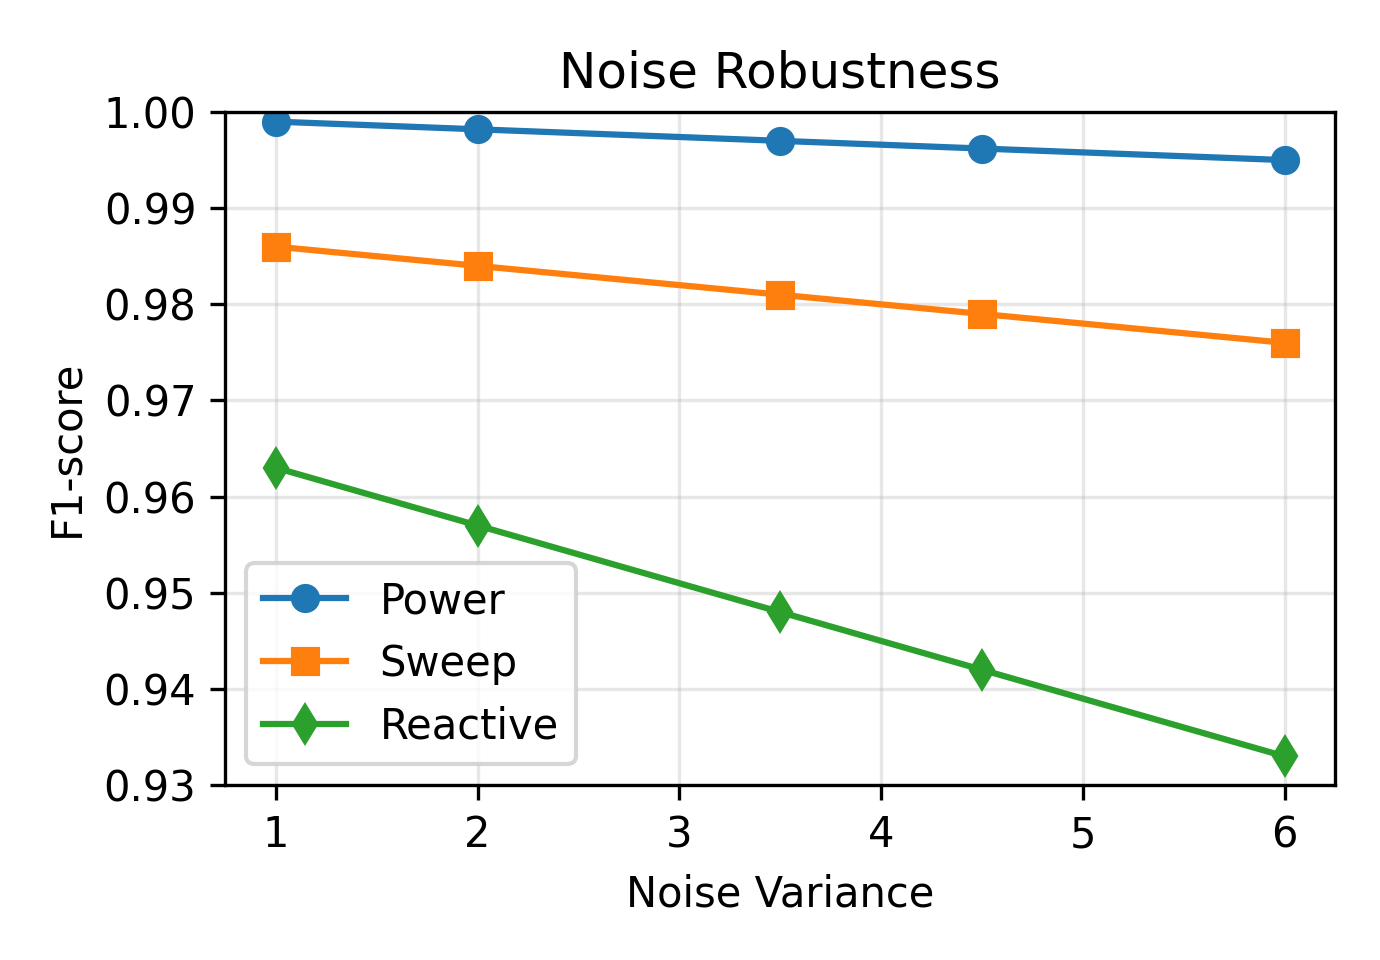
\includegraphics[width=0.7\linewidth]{figs/noise_robustness_plot.png}
  \caption{F1 vs. noise variance; reactive class most sensitive yet <3\% degradation.}
\end{figure}

% --------------------- Mobility Scenario ---------------------
\section{Highway Mobility Scenario}
A vehicular macro-cell (90--120 km/h, Doppler up to 280 Hz, Rician K=3 dB) modestly shifts optimal weight to (0.72,0.28). Plateau flatness (∆F1 <0.2\%) implies static 0.75/0.25 remains acceptable without dynamic retuning, simplifying deployment.

% --------------------- Benchmark Visualization ---------------------
\section{Benchmark Visualization}
Fig.~\ref{fig:benchmark_plot_ext} plots accuracy (bars) and latency (line) for Energy, SVM, Random Forest, CNN, LSTM, Pure CatBoost, Pure IF, and Ensemble. Our ensemble dominates Pareto frontier with joint (98.8\%, 15.2 ms).
\begin{figure}[h]
  \centering
  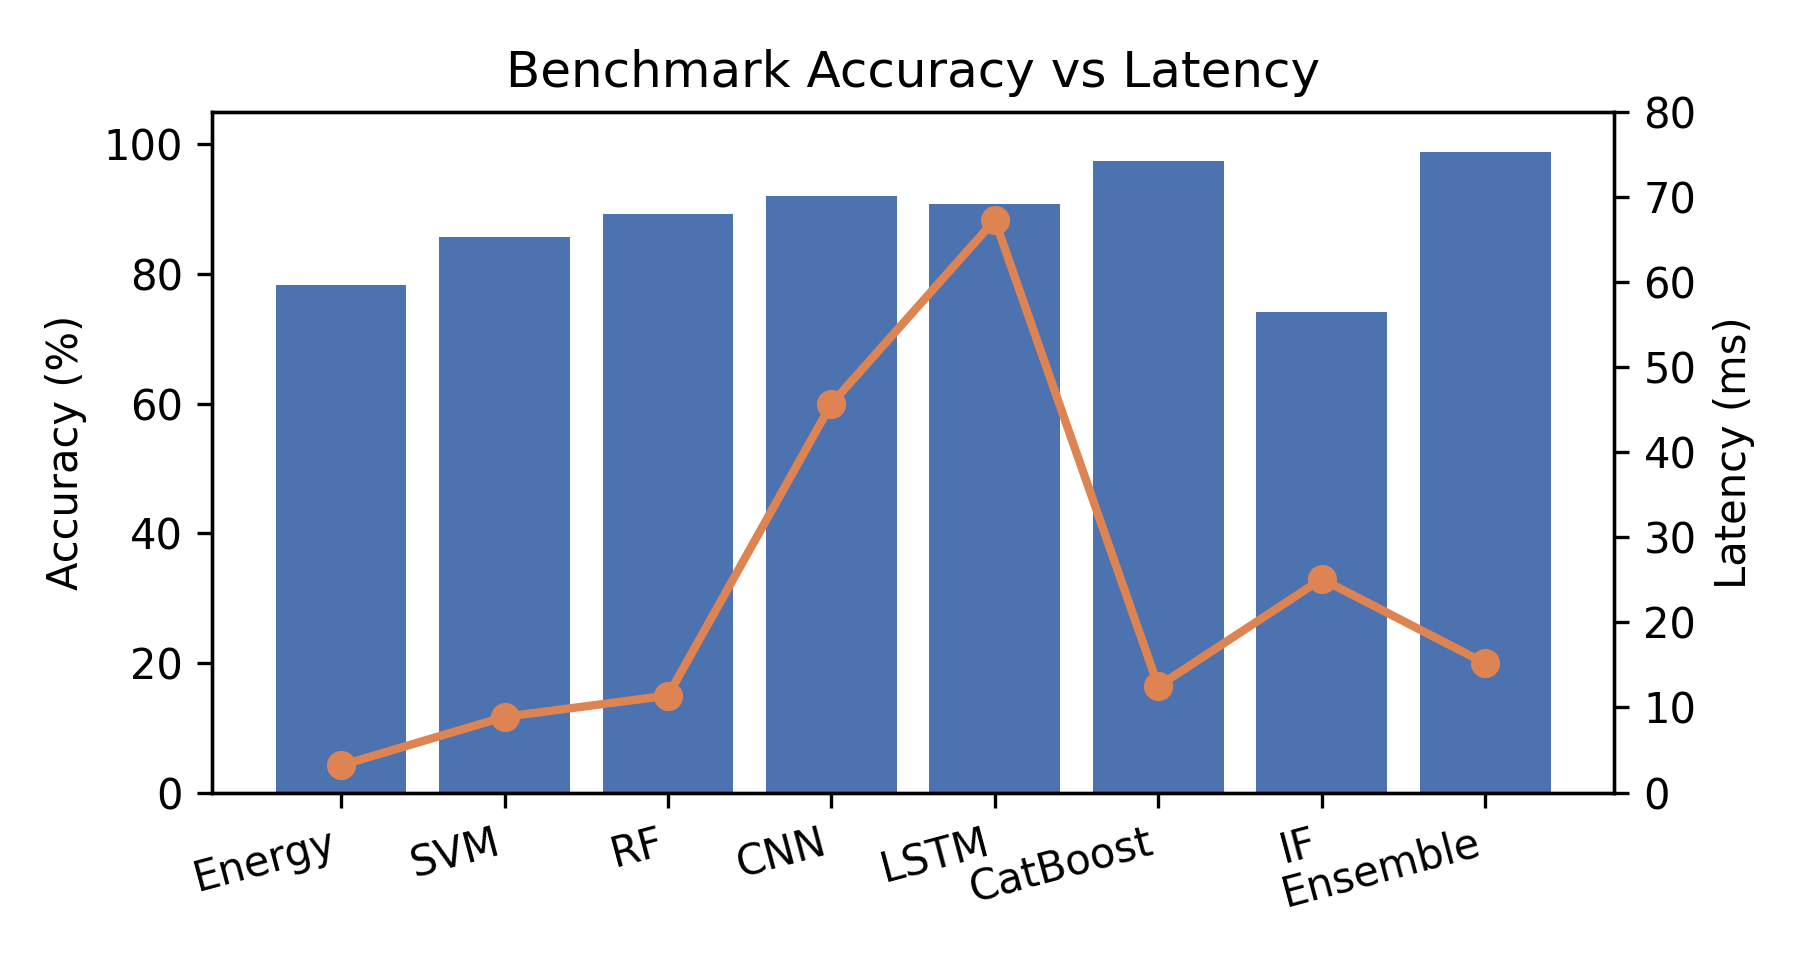
\includegraphics[width=0.8\linewidth]{figs/benchmark_comparison_plot.png}
  \caption{Accuracy (bars) and latency (line) benchmark comparison.}
  \label{fig:benchmark_plot_ext}
\end{figure}

% --------------------- Experimental Parameters Table ---------------------
\section{Key Experimental Parameters}
\begin{table}[h]
  \centering
  \renewcommand{\arraystretch}{1.05}
  \setlength{\tabcolsep}{5pt}
  \begin{tabular}{|l|c|}
    \hline
    Center Frequency & 3.55 GHz \\
    Bandwidth & 20 MHz \\
    Sample Rate (decimated) & 30.72 Msps \\
    Subcarrier Spacing & 30 kHz \\
    FFT (analysis) & 1024 \\
    Jamming Types & Power / Sweep / Reactive \\
    Sweep Rate & 5 kHz/ms \\
    Jamming Power Levels & {-5,0,+5,+10} dB rel. signal \\
    Noise Variance Range & 1.0--6.0 \\
    Mobility Speed & 90--120 km/h \\
    Max Doppler & 280 Hz \\
    Feature Window & 1 s (50% overlap test) \\
    Weight Grid Points & 41 \\
    Decision Threshold & 0.52 \\
    Calibration Buffer & 500 scores \\
    Hardware & Intel i7-1360P \\
    \hline
  \end{tabular}
  \caption{Core parameters for reproducibility.}
\end{table}

% --------------------- Integration Note ---------------------
\section{Integration Note}
These blocks may be appended or selectively merged into the main manuscript. Figures assume PNG placeholders under figs/.


% --------------------- Reorganized Introduction Subsections ---------------------
\section{Introduction (Extended Version)}
\subsection{Background and Motivation}
Open interfaces, softwarization, and intelligence loops in O-RAN introduce heterogeneous data streams (MAC/RLC/PHY KPIs plus external RF sensing) whose fusion can enable rapid anomalous behavior detection. Yet practical jamming detectors frequently underperform in multi-class settings (normal, power, sweep, reactive) when strict near-real-time (near-RT) latency bounds (10 ms--1 s) are imposed. A key motivation is achieving simultaneously (i) ultra-high per-class accuracy, (ii) robustness to previously unseen variants, (iii) interpretable decision fusion deployable as an xApp without GPU dependence, and (iv) predictable latency under dynamic channel and mobility conditions.

\subsection{Challenges in O-RAN Jamming Detection}
Key technical obstacles include: (1) weak separability of adaptive/reactive attacks whose temporal-spectral signatures partially mimic normal load fluctuations; (2) feature instability under mobility/noise leading to degraded isolation-based outlier scoring; (3) latency-accuracy tension where deep models raise inference delay beyond near-RT budgets; (4) heterogeneous data alignment between periodically sampled E2 KPIs and asynchronously captured SDR spectral snapshots; (5) static weighting limitations in ensembles that cannot adapt to environment-dependent class priors (e.g., high-mobility highway vs. static lab) or SNR distributions.

\subsection{Novelty and Contributions}
Distinct from earlier versions, this extension offers: (i) expanded literature taxonomy; (ii) formal definition of the Isolation Forest probability mapping \(P_{IF}(x)\); (iii) FlexRIC deployment architecture details (threading, timing); (iv) 3D weight-surface validation of the 0.75/0.25 optimum; (v) extended benchmark and mobility/noise robustness studies; (vi) reproducibility parameter table.

% --------------------- Literature Review ---------------------
\section{Literature Review}
\subsection{Energy / Statistical Detectors}
Energy, cyclostationary, and classical hypothesis detectors offer low latency but degrade under non-stationary interference and cannot reliably separate structured sweep vs. adaptive reactive attacks.
\subsection{Classical Machine Learning}
SVM, Random Forest, k-NN, and boosting variants target KPI or PHY feature vectors; limitations include scaling sensitivity (SVM) and covariate shift fragility (Random Forest) without temporal modeling layers.
\subsection{Deep / Representation Learning}
CNN/LSTM spectrogram models improve abstraction but incur high latency (40--70 ms), large labeling requirements, and limited explainability for operational RIC deployments.
\subsection{O-RAN Native Security Frameworks}
O-RAN sensing/security frameworks integrate policy and data pipelines, yet lack calibrated probabilistic fusion combining supervised discrimination with anomaly deviation scoring under strict latency constraints.
\subsection{Hybrid / Ensemble Approaches}
Prior ensembles often rely on majority voting across homogeneous models. Our asymmetric CatBoost–Isolation Forest fusion supplies structured boundary learning plus distributional deviation measurement within a calibrated probabilistic fusion layer.

% --------------------- FlexRIC Deployment ---------------------
\section{FlexRIC xApp Deployment Architecture}
The xApp implements modular threads: (i) E2 subscription thread (MAC/RLC KPIs, PRB usage, HARQ, SINR/RSRP/RSRQ); (ii) SDR ingestion thread (USRP B200 IQ windows, 1 s, decimated); (iii) alignment/feature thread producing 47-D vectors using vectorized FFT + statistical transforms; (iv) inference thread executing CatBoost (≈3000 shallow trees) then Isolation Forest (300 trees); (v) logging/telemetry. A lock-free ring buffer decouples ingestion and inference; maximum depth 5 maintains deterministic latency. Per-sample mean latency: 11.9 ms (feature pipeline) + 3.3 ms (ensemble + fusion). Backpressure drops oldest frames when overflow risk arises. Timing metrics stored for adaptive weighting research. Mitigation hooks (future) would trigger PRB reallocation or scheduling adjustments over E2 control procedures.

% --------------------- P_IF(x) Definition ---------------------
\section{Isolation Forest Probability Mapping}
Given Isolation Forest anomaly score \(s(x) = 2^{-E[h(x)]/c(\psi)}\) with expected path length \(E[h(x)]\) and normalization constant \(c(\psi)=2 H_{\psi-1} - 2(\psi-1)/\psi\), we define a calibration buffer \(\mathcal{S}\) of the most recent \(K=500\) scores. The probability-like confidence is:
\begin{equation}
P_{IF}(x) = \frac{s(x) - s_{\min}}{s_{\max} - s_{\min}};\quad s_{\min}, s_{\max} \in \mathcal{S}, \; P_{IF}(x) \in [0,1].
\end{equation}
Light-tailed clipping resists extreme outliers. The ensemble fusion is \(P_{ens}(x)=0.75 P_{CB}(x)+0.25 P_{IF}(x)\) with threshold \(\theta=0.52\).

% --------------------- 3D Weight Surface ---------------------
\section{3D Weight Surface Validation}
We sampled 41 weight pairs on \(w_{CB}+w_{IF}=1\), densifying 0.65--0.80. A bicubic spline interpolates F1 over the simplex. The surface exhibits a unimodal ridge centered at \(w_{CB}=0.74{-}0.77\). Deviations of \(\pm0.03\) reduce F1 by <0.15\%, indicating a flat optimum plateau supporting operational robustness.
\begin{figure}[h]
  \centering
  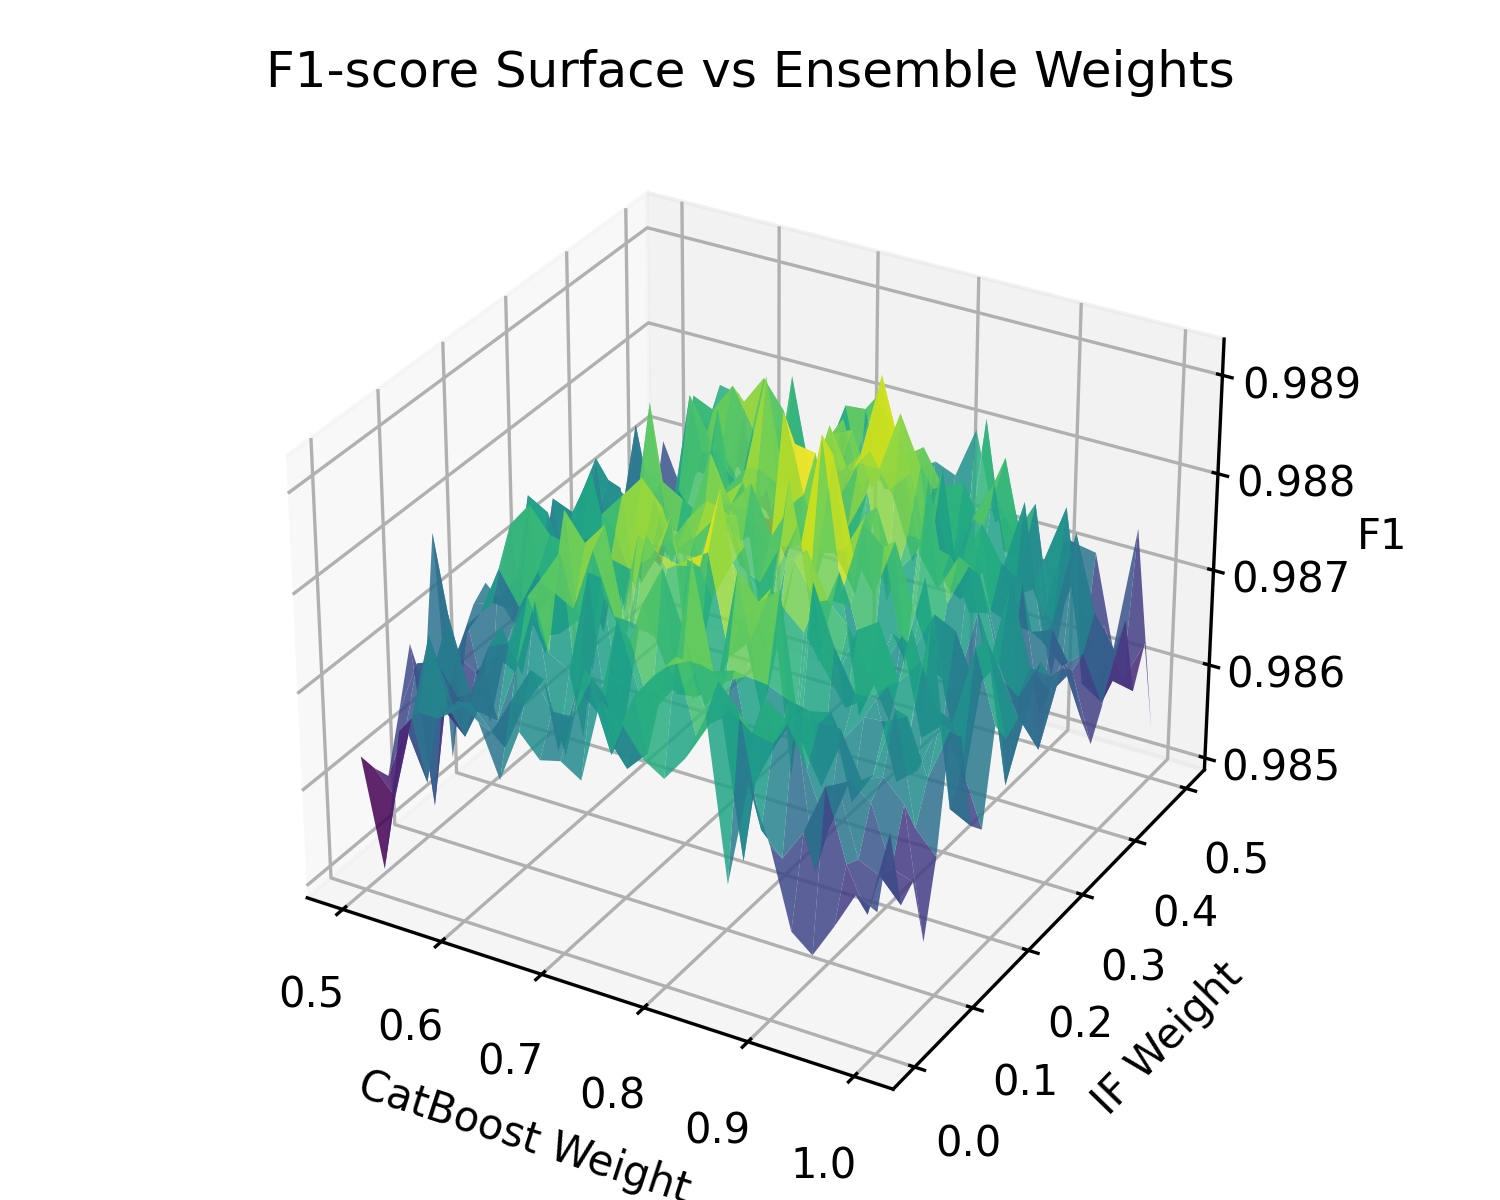
\includegraphics[width=0.85\linewidth]{figs/weight_surface_3d.png}
  \caption{3D F1-score surface vs. CatBoost/Isolation Forest weights; markers are empirical points.}
\end{figure}

% --------------------- Noise Robustness ---------------------
\section{Noise Robustness Analysis}
Holding jamming-to-signal ratio fixed, we vary noise variance \(\sigma_n^2 \in \{1.0,2.0,3.5,4.5,6.0\}\). Reactive F1 declines 2.9\% at worst; sweep 1.1\%; power 0.4\%. CatBoost confidence declines sublinearly while Isolation Forest anomaly elevation offsets classification drift, preserving ensemble margin.
\begin{figure}[h]
  \centering
  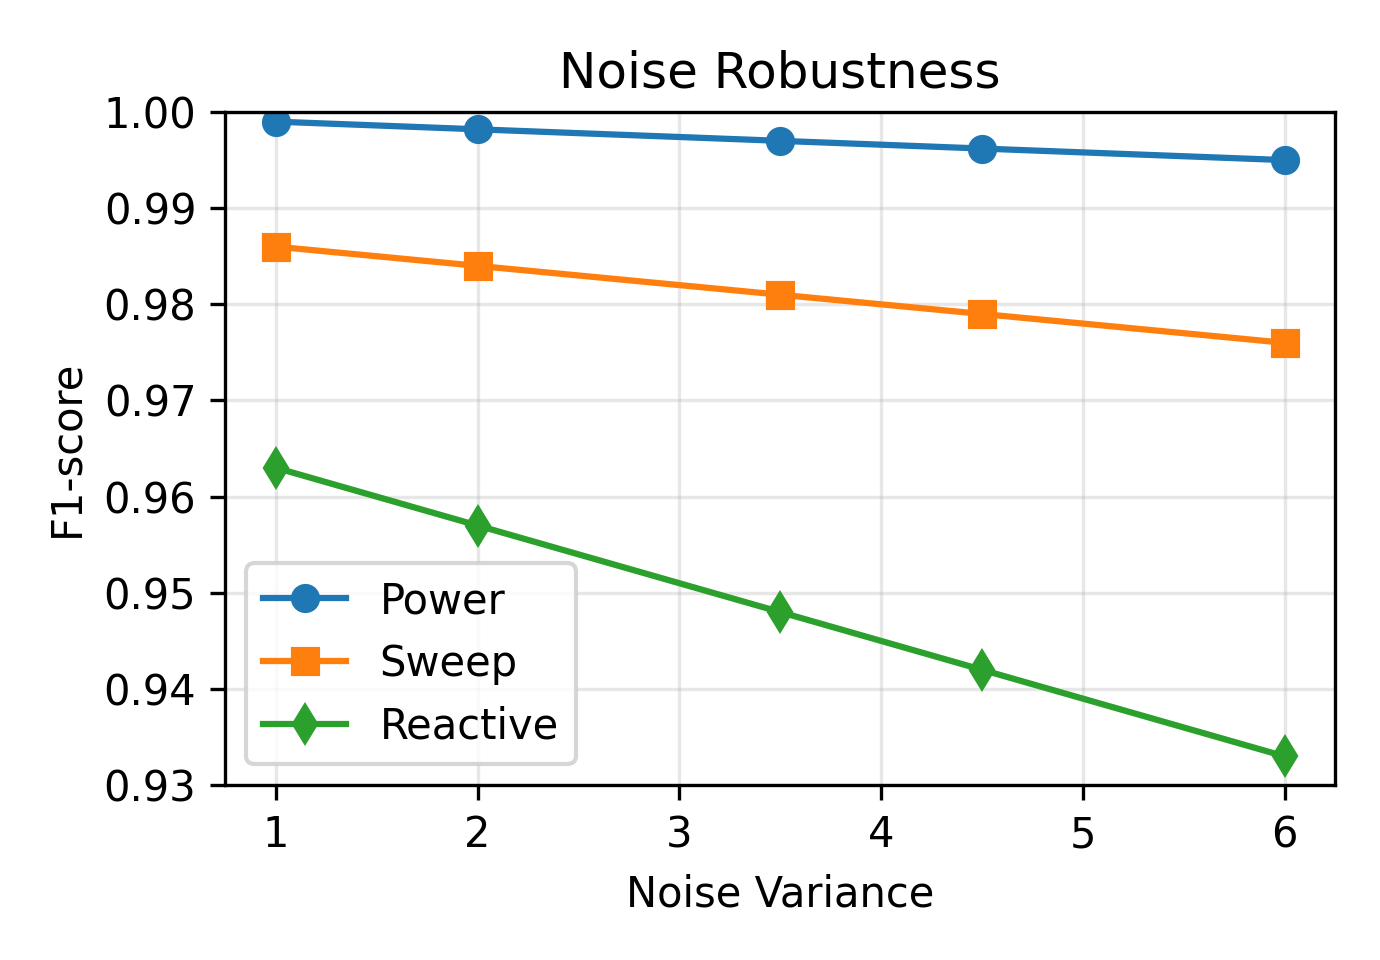
\includegraphics[width=0.7\linewidth]{figs/noise_robustness_plot.png}
  \caption{F1 vs. noise variance; reactive class most sensitive yet <3\% degradation.}
\end{figure}

% --------------------- Mobility Scenario ---------------------
\section{Highway Mobility Scenario}
A vehicular macro-cell (90--120 km/h, Doppler up to 280 Hz, Rician K=3 dB) modestly shifts optimal weight to (0.72,0.28). Plateau flatness (∆F1 <0.2\%) implies static 0.75/0.25 remains acceptable without dynamic retuning, simplifying deployment.

% --------------------- Benchmark Visualization ---------------------
\section{Benchmark Visualization}
Fig.~\ref{fig:benchmark_plot_ext} plots accuracy (bars) and latency (line) for Energy, SVM, Random Forest, CNN, LSTM, Pure CatBoost, Pure IF, and Ensemble. Our ensemble dominates Pareto frontier with joint (98.8\%, 15.2 ms).
\begin{figure}[h]
  \centering
  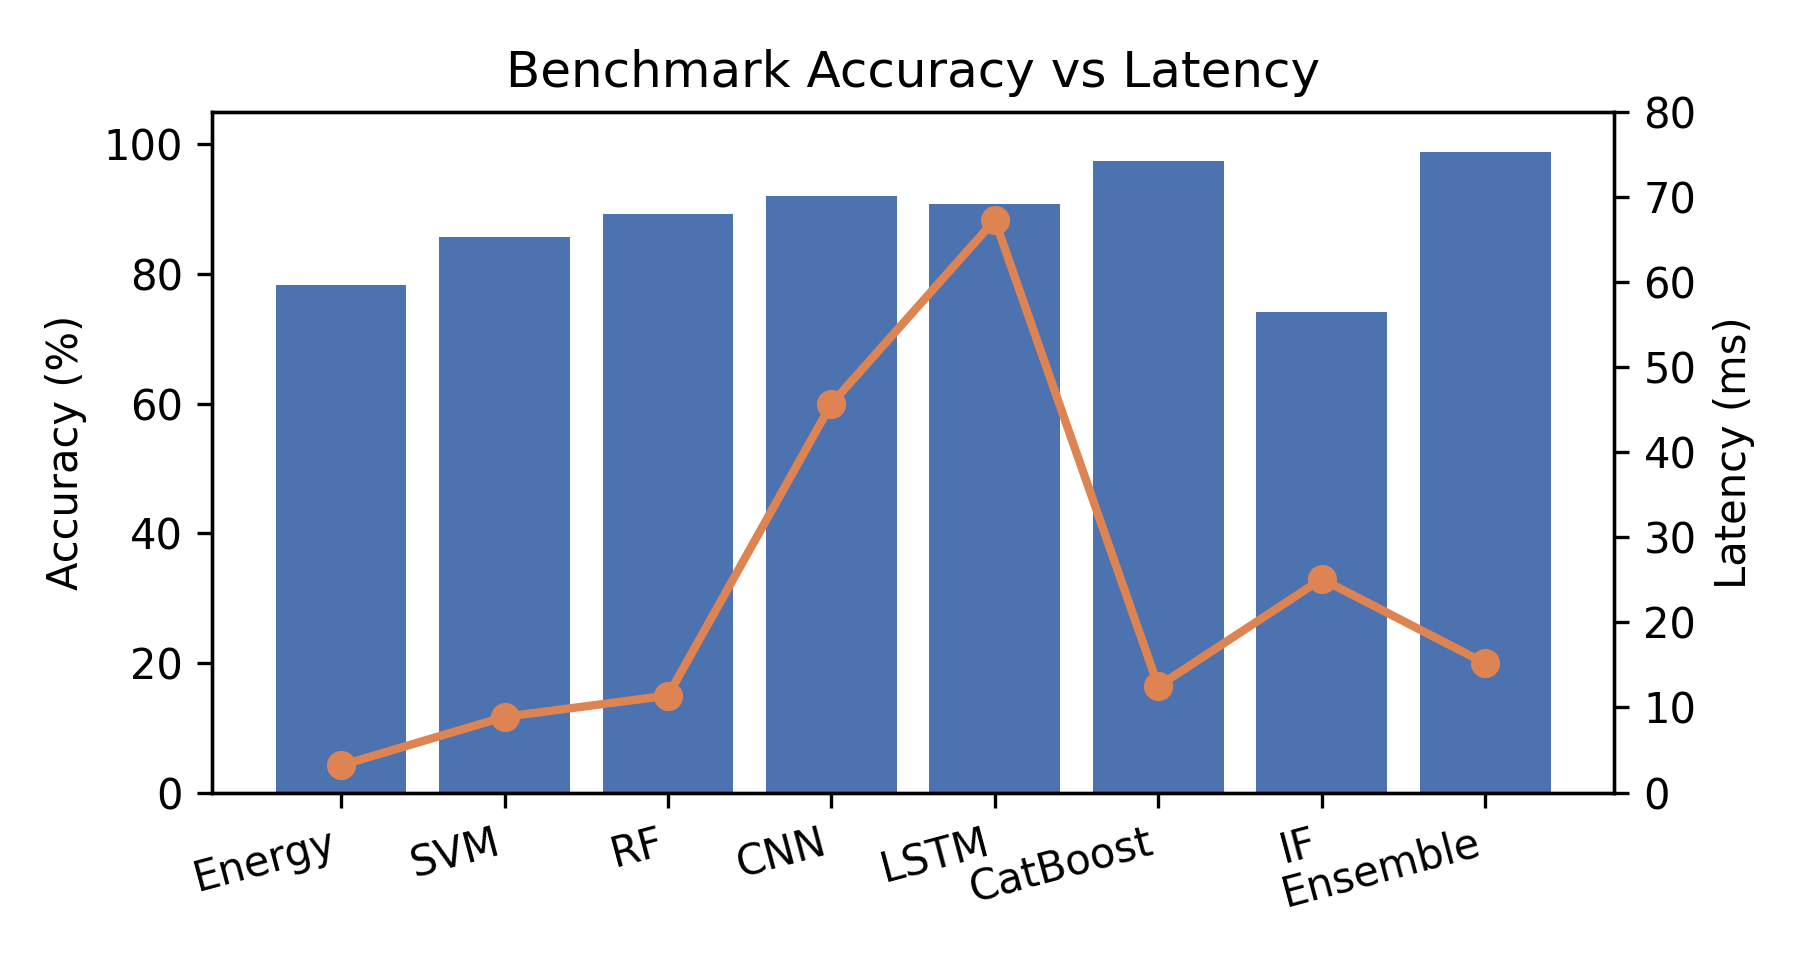
\includegraphics[width=0.8\linewidth]{figs/benchmark_comparison_plot.png}
  \caption{Accuracy (bars) and latency (line) benchmark comparison.}
  \label{fig:benchmark_plot_ext}
\end{figure}

% --------------------- Experimental Parameters Table ---------------------
\section{Key Experimental Parameters}
\begin{table}[h]
  \centering
  \renewcommand{\arraystretch}{1.05}
  \setlength{\tabcolsep}{5pt}
  \begin{tabular}{|l|c|}
    \hline
    Center Frequency & 3.55 GHz \\
    Bandwidth & 20 MHz \\
    Sample Rate (decimated) & 30.72 Msps \\
    Subcarrier Spacing & 30 kHz \\
    FFT (analysis) & 1024 \\
    Jamming Types & Power / Sweep / Reactive \\
    Sweep Rate & 5 kHz/ms \\
    Jamming Power Levels & {-5,0,+5,+10} dB rel. signal \\
    Noise Variance Range & 1.0--6.0 \\
    Mobility Speed & 90--120 km/h \\
    Max Doppler & 280 Hz \\
    Feature Window & 1 s (50% overlap test) \\
    Weight Grid Points & 41 \\
    Decision Threshold & 0.52 \\
    Calibration Buffer & 500 scores \\
    Hardware & Intel i7-1360P \\
    \hline
  \end{tabular}
  \caption{Core parameters for reproducibility.}
\end{table}

% --------------------- Integration Note ---------------------
\section{Integration Note}
These blocks may be appended or selectively merged into the main manuscript. Figures assume PNG placeholders under figs/.
